\documentclass[nobib]{tufte-handout}

%\\geometry{showframe}% for debugging purposes -- displays the margins
\usepackage{amssymb}
\usepackage{hyperref}
\usepackage{pgfplots}
\usepackage[activate={true,nocompatibility},final,tracking=true,kerning=true,spacing=true,factor=1100,stretch=10,shrink=10]{microtype}
\usepackage{color}
\usepackage{steinmetz}
\usepackage{placeins}
\usepackage{marginfix}
\usepackage{array}
\usepackage{tikz}
\usepackage{amsmath}
\usepackage{amsthm}
\usetikzlibrary{shapes}
\usetikzlibrary{positioning}
\usepackage{listings}
\usepackage[edges]{forest}
\usepackage{caption}
\usepackage[T1]{fontenc}
\usepackage{lmodern}
\DeclareCaptionFont{white}{\color{white}}
\DeclareCaptionFormat{listing}{\colorbox{gray}{\parbox{\textwidth}{#1#2#3}}}
\captionsetup[lstlisting]{format=listing,labelfont=white,textfont=white}

% Set up the images/graphics package
\usepackage{graphicx}
\setkeys{Gin}{width=\linewidth,totalheight=\textheight,keepaspectratio}
\graphicspath{{.}}

\title{Notes for ECE 36800 - Data Structures}
\author{Zeke Ulrich}
\date{\today}  % if the \date{} command is left out, the current date will be used

% The following package makes prettier tables.  We're all about the bling!
\usepackage{booktabs}

% The units package provides nice, non-stacked fractions and better spacing
% for units.
\usepackage{units}

% The fancyvrb package lets us customize the formatting of verbatim
% environments.  We use a slightly smaller font.
\usepackage{fancyvrb}
\fvset{fontsize=\normalsize}

% Small sections of multiple columns
\usepackage{multicol}

% For finite state machines 
\usetikzlibrary{automata} % Import library for drawing automata
\usetikzlibrary{positioning} % ...positioning nodes
\usetikzlibrary{arrows} % ...customizing arrows
\tikzset{node distance=2.5cm, % Minimum distance between two nodes. Change if necessary.
    every state/.style={ % Sets the properties for each state
    semithick,
    fill=gray!10},
    initial text={}, % No label on start arrow
    double distance=2pt, % Adjust appearance of accept states
    every edge/.style={ % Sets the properties for each transition
    draw,
    ->,>=stealth', % Makes edges directed with bold arrowheads
    auto,
    semithick}}
\let\epsilon\varepsilon

% These commands are used to pretty-print LaTeX commands
\newcommand{\doccmd}[1]{\texttt{\textbackslash#1}}% command name -- adds backslash automatically
\newcommand{\docopt}[1]{\ensuremath{\langle}\textrm{\textit{#1}}\ensuremath{\rangle}}% optional command argument
\newcommand{\docarg}[1]{\textrm{\textit{#1}}}% (required) command argument
\newenvironment{docspec}{\begin{quote}\noindent}{\end{quote}}% command specification environment
\newcommand{\docenv}[1]{\textsf{#1}}% environment name
\newcommand{\docpkg}[1]{\texttt{#1}}% package name
\newcommand{\doccls}[1]{\texttt{#1}}% document class name
\newcommand{\docclsopt}[1]{\texttt{#1}}% document class option name

% Define a custom command for definitions and biconditional
\newcommand{\defn}[2]{\noindent\textbf{#1}:\ #2}
\let\biconditional\leftrightarrow

\begin{document}

\maketitle

\tableofcontents

\section{Course Description}
Provides insight into the use of data structures.
Topics include stacks, queues and lists, trees,
graphs, sorting, searching, and hashing.
\pagebreak

\section{Introduction}
Let's examine some basic C++ programs.
\begin{lstlisting}[language=C++,caption=Hello World]
    #include <iostream>

    int main() {
        std::cout << "Hello World!";
        return 0;
    }
\end{lstlisting}

\begin{lstlisting}[language=C++,caption=User Input]
    #include <iostream>

    int main() {
        double n;
        int i;

        std::cout << "Enter float: ";
        std::cin >> n;

        std::cout << "Enter integer: ";
        std::cin >> i;

        return 0;
    }
\end{lstlisting}

The \texttt{stds} you're seeing all over the place refer not
to a frat party but the standard namespace. It holds
useful objects like standard in ("\texttt{cin}") and standard
out ("\texttt{cout}").

In C, we use \texttt{malloc} and \texttt{free} to allocate memory. In C++,
the equivalent operations are \texttt{new} and \texttt{delete}.

\begin{lstlisting}[language=C++,caption=Free and Delete]
    void CorrectUsage(){
        int *ptr = new int[3];
        int *ptr1 = new int;
        ptr[0] = 1;
        ptr[1] = 2;
        ptr[2] = 3;
        *ptr1 = 5;
        delete ptr1;
        delete [] ptr;        
\end{lstlisting}
The reason for this is using \texttt{new} and \texttt{free} calls
an object's constructor and destructors, which are defined to properly
delete the object. Technically, \texttt{malloc} and \texttt{free} are
both present in C++, but they won't trigger the constructors and
destructors and should be avoided. The choice to leave these functions in
was made to improve compatibility with C, which is a theme the reader
may notice in C++'s many possible ways to do the same thing.

C++ filenames are terminated with a \texttt{.cpp} or \texttt{.cc}
extension, like \texttt{example.cpp} or \texttt{example.cc}
\section{Sorting}
\subsection{Bubble Sort}
Bubble Sort is a simple sorting algorithm that repeatedly steps 
through the list, compares adjacent elements, and swaps them if 
they are in the wrong order. The pass through the list is repeated 
until the list is sorted.

\textbf{Time Complexity:}
\begin{itemize}
    \item Best Case: $O(n)$ (when the array is already sorted)
    \item Average Case: $O(n^2)$
    \item Worst Case: $O(n^2)$
\end{itemize}

\begin{lstlisting}[caption=Bubble Sort]
void bubble_sort(int arr[], int n) {
    for (int i = 0; i < n-1; i++) {
        int swapped = 0;
        for (int j = 0; j < n-i-1; j++) {
            if (arr[j] > arr[j+1]) {
                int temp = arr[j];
                arr[j] = arr[j+1];
                arr[j+1] = temp;
                swapped = 1;
            }
        }
        if (swapped == 0)
            break;
    }
}
\end{lstlisting}
\subsection{Insertion Sort}
Insertion Sort builds the sorted array one item at a time. 
It picks an element and places it into its correct position in 
the sorted part of the array.

\textbf{Time Complexity:}
\begin{itemize}
    \item Best Case: $O(n)$ (when the array is already sorted)
    \item Average Case: $O(n^2)$
    \item Worst Case: $O(n^2)$
\end{itemize}

\begin{lstlisting}[caption=Insertion Sort]
void insertion_sort(int arr[], int n) {
    for (int i = 1; i < n; i++) {
        int key = arr[i];
        int j = i - 1;
        while (j >= 0 && arr[j] > key) {
            arr[j + 1] = arr[j];
            j = j - 1;
        }
        arr[j + 1] = key;
    }
}
\end{lstlisting}
\subsection{Selection Sort}
Selection Sort divides the array into a sorted and an unsorted 
region. It repeatedly selects the smallest (or largest) element 
from the unsorted region and moves it to the sorted region.

\textbf{Time Complexity:}
\begin{itemize}
    \item Best Case: $O(n^2)$
    \item Average Case: $O(n^2)$
    \item Worst Case: $O(n^2)$
\end{itemize}

\begin{lstlisting}[caption=Selection Sort]
void selection_sort(int arr[], int n) {
    for (int i = 0; i < n-1; i++) {
        int min_idx = i;
        for (int j = i+1; j < n; j++) {
            if (arr[j] < arr[min_idx])
                min_idx = j;
        }
        int temp = arr[min_idx];
        arr[min_idx] = arr[i];
        arr[i] = temp;
    }
}
\end{lstlisting}
\subsection{Shell Sort}
Shell Sort is an optimization over Insertion Sort. 
It first sorts elements that are far apart and then progressively 
reduces the gap between elements to be sorted.

\textbf{Time Complexity:}
\begin{itemize}
    \item Best Case: $O(n \log n)$
    \item Average Case: depends on the gap sequence, commonly $O(n^{3/2})$ or $O(n \log^2 n)$
    \item Worst Case: $O(n^2)$
\end{itemize}

\begin{lstlisting}[caption=Shell Sort]
void shell_sort(int arr[], int n) {
    for (int gap = n/2; gap > 0; gap /= 2) {
        for (int i = gap; i < n; i++) {
            int temp = arr[i];
            int j;
            for (j = i; j >= gap && arr[j - gap] > temp; j -= gap) {
                arr[j] = arr[j - gap];
            }
            arr[j] = temp;
        }
    }
}
\end{lstlisting}
\section{Asymptotic Notation}

\subsection{Big O}
Big $O$ notation describes the upper bound 
of an algorithm's growth rate. It provides an 
asymptotic measure of the time complexity or 
space complexity of an algorithm as a function of 
the input size. Informally, big $O$ notation
just picks out the highest 
order term from your runtime expression. 
Formally, Big $O$ is defined as follows:
\[
f(n) \in O(g(n)) \iff \exists \, c > 0 \text{ and } n_0 \geq 0 \text{ such that } \forall n \geq n_0, \, 0 \leq f(n) \leq c \cdot g(n).
\]
\begin{itemize}
    \item $f(n)$: The function representing the actual growth rate of the algorithm.
    \item $g(n)$: The comparison function, often representing the dominant term of $f(n)$.
    \item $c > 0$: A constant that scales $g(n)$ to bound $f(n)$.
    \item $n_0$: A constant representing the threshold beyond which the inequality holds.
\end{itemize}

Big $O$ notation focuses on the dominant term of $g(n)$, 
ignoring lower-order terms and constant factors, to provide a 
simplified representation of the algorithm's efficiency.

\subsection{Big $\Omega$}
Big $\Omega$ notation describes the lower bound 
of an algorithm's growth rate. It provides an 
asymptotic measure of the minimum time complexity or 
space complexity of an algorithm as a function of 
the input size. While Big $O$ focuses on the upper bound, 
Big $\Omega$ focuses on the lower bound, ensuring that the 
algorithm's growth rate is at least as fast as a specified 
function, up to constant factors. Formally, Big $\Omega$ is defined as follows:
\[
f(n) \in \Omega(g(n)) \iff \exists \, c > 0 \text{ and } n_0 \geq 0 \text{ such that } \forall n \geq n_0, \, 0 \leq c \cdot g(n) \leq f(n).
\]
\begin{itemize}
    \item $f(n)$: The function representing the actual growth rate of the algorithm.
    \item $g(n)$: The comparison function, representing the lower bound on $f(n)$.
    \item $c > 0$: A constant that scales $g(n)$ to bound $f(n)$ from below.
    \item $n_0$: A constant representing the threshold beyond which the inequality holds.
\end{itemize}

Big $\Omega$ notation is used to describe the best-case or 
minimum growth rate of an algorithm. For example, if an 
algorithm's runtime is $\Omega(n \log n)$, it means that the 
algorithm cannot perform better than $n \log n$ in the best case, 
up to constant factors. This notation is particularly useful 
when proving lower bounds on the complexity of problems or algorithms.

\subsection{Big $\Theta$}
Big $\Theta$ notation describes both the upper and lower bounds 
of an algorithm's growth rate. It provides a tight asymptotic 
bound on the time complexity or space complexity of an algorithm 
as a function of the input size. Unlike Big $O$, which only provides 
an upper bound, Big $\Theta$ ensures that the growth rate of the 
algorithm is bounded both above and below by the same function, 
up to constant factors. Formally, Big $\Theta$ is defined as follows:
\[
f(n) \in \Theta(g(n)) \iff \exists \, c_1, c_2 > 0 \text{ and } n_0 \geq 0 \text{ such that } \forall n \geq n_0, \, c_1 \cdot g(n) \leq f(n) \leq c_2 \cdot g(n).
\]
\begin{itemize}
    \item $f(n)$: The function representing the actual growth rate of the algorithm.
    \item $g(n)$: The comparison function, representing the tight bound on $f(n)$.
    \item $c_1, c_2 > 0$: Constants that scale $g(n)$ to bound $f(n)$ from below and above.
    \item $n_0$: A constant representing the threshold beyond which the inequality holds.
\end{itemize}

Big $\Theta$ notation is used when the growth rate of an algorithm 
is known to be tightly constrained by a specific function, providing 
a precise characterization of its efficiency. For example, if an 
algorithm's runtime is both $O(n^2)$ and $\Omega(n^2)$, then its 
runtime is $\Theta(n^2)$.
\section{Recursion}

The fundemental components of recursion are
\begin{enumerate}
    \item A base case (or base cases)
    \item A method to split the problem into smaller, similar problems.
\end{enumerate}

\subsection{Master Theorem}

The Master Theorem provides a method for solving recurrence relations
of the form:
\[
    T(n) = aT\left(\frac{n}{b}\right) + f(n)
\]
where:
\begin{itemize}
    \item \( a \geq 1 \) is the number of subproblems in the recursion,
    \item \( b > 1 \) is the factor by which the problem
          size is reduced in each recursive call,
    \item \( f(n) \) is the cost of the work done outside
          the recursive calls, including the cost of dividing the problem and merging results.
\end{itemize}

The theorem provides asymptotic bounds on \( T(n) \)
based on the relationship between \( f(n) \) and \( n^{\log_b a} \).

The asymptotic behavior of \( T(n) \) is determined
by comparing \( f(n) \) with \( n^{\log_b a} \):

\textbf{Case 1: Polynomially Smaller Work at Each Level}

If \( f(n) = O(n^c) \) for some constant \( c < \log_b a \), then:

\[
    T(n) = \Theta(n^{\log_b a})
\]

\textbf{Explanation:} The total cost is dominated by the recursive term, meaning the majority of the work is done at the top levels of recursion.

\textbf{Case 2: Balanced Work at All Levels}

If \( f(n) = \Theta(n^{\log_b a}) \), then:

\[
    T(n) = \Theta(n^{\log_b a} \log n)
\]

\textbf{Explanation:} The work done at each level is roughly the same, so the logarithmic factor arises from the accumulation of work over all levels.

\textbf{Case 3: Work Dominated by the Non-Recursive Term}

If \( f(n) = \Omega(n^c) \) for some constant \( c > \log_b a \), and if the regularity condition holds:

\[
    a f\left(\frac{n}{b}\right) \leq c_1 f(n) \quad \text{for some } c_1 < 1 \text{ and sufficiently large } n,
\]

then:

\[
    T(n) = \Theta(f(n))
\]

\textbf{Explanation:} The majority of the work is done at the base
level of recursion rather than at the top, meaning \( f(n) \)
dominates the total complexity.

\textbf{Example 1: Merge Sort}

The recurrence relation for Merge Sort is:

\[
    T(n) = 2T\left(\frac{n}{2}\right) + O(n)
\]

Here, \( a = 2 \), \( b = 2 \), and \( f(n) = O(n) \). We compare \( f(n) \) with \( n^{\log_2 2} = n \). Since \( f(n) = \Theta(n^{\log_2 2}) \), Case 2 applies:

\[
    T(n) = \Theta(n \log n)
\]

\textbf{Example 2: Binary Search}

The recurrence relation for Binary Search is:

\[
    T(n) = T\left(\frac{n}{2}\right) + O(1)
\]

Here, \( a = 1 \), \( b = 2 \), and \( f(n) = O(1) \). We compare \( f(n) \) with \( n^{\log_2 1} = n^0 = 1 \). Since \( f(n) = O(n^c) \) with \( c = 0 < \log_2 1 = 0 \), Case 1 applies:

\[
    T(n) = \Theta(\log n)
\]

\subsection{Recursion Limit}

Recursive solutions can reach the max recursive depth and
terminate your program early. The way to avoid this is with
an iterative solution. Taking the example of the Fibonacci
sequence, you could implement it as in listing \ref{lst:fib}

\begin{lstlisting}[language=C, label={lst:fib}, caption=Singly Linked List Node Structure]
    #include <stdio.h>

    // Function to calculate the nth Fibonacci number using recursion
    int nthFibonacci(int n){
        // Base case: if n is 0 or 1, return n
        if (n <= 1){
            return n;
        }
        // Recursive case: sum of the two preceding numbers
        return nthFibonacci(n - 1) + nthFibonacci(n - 2);
    }

    int main(){
        int n = 5;
        int result = nthFibonacci(n);
        printf("%d\n", result);
        return 0;
    }
\end{lstlisting}

However, the runtime increases exponentially.
\marginnote{In fact, the runtime increases as $\Phi^n$, where
    $\Phi$ is the golden ratio.}
There is a much better solution, an iterative one.
For listing \ref{lst:fibit} the time complexity is $O(n)$
instead of $O(2^n)$.

\begin{lstlisting}[language=C, label={lst:fibit}, caption=Singly Linked List Node Structure]
    #include <math.h>
    #include <stdio.h>

    // Approximate value of golden ratio
    double PHI = 1.6180339;

    // Fibonacci numbers upto n = 5
    int f[6] = { 0, 1, 1, 2, 3, 5 };

    int fib(int n)
    {
        // Fibonacci numbers for n < 6
        if (n < 6)
            return f[n];

        // Else start counting from
        // 5th term
        int t = 5, fn = 5;

        while (t < n) {
            fn = round(fn * PHI);
            t++;
        }

        return fn;
    }

    int main()
    {
        int n = 9;
        printf("%d th Fibonacci Number = %d\n", n, fib(n));
        return 0;
    }
\end{lstlisting}

\subsection{Space Complexity}

The space complexity of a recursive function is proportional to
the depth of the computation tree, since that gives us the longest
possible path (read: the highest number of frames on the call stack).
For instance, if each frame has a space complexity of $n$, and the
computation tree has a depth of $\log_2(n)$, the space complexity
of the algorithm is $O(n\log(n))$.

\subsection{Tail Recursion}
Tail recursion is a special case of recursion where the recursive
call is the last operation performed in a function before returning
the result. Tail recursion can be transformed into iteration, and in
some languages this is done automatically under the hood.

\begin{lstlisting}[language=C, caption={Regular Recursion}]
    #include <stdio.h>

    int factorial(int n) {
        if (n == 0)
            return 1;
        return n * factorial(n - 1);  
        // Multiplication happens after recursive call
    }

    int main() {
        printf("%d\n", factorial(5)); // Output: 120
        return 0;
    }
\end{lstlisting}

\begin{lstlisting}[language=C, caption={Tail Recursion}, label={lst:tailrecursion}]
    #include <stdio.h>

    int factorial_helper(int n, int acc) {
        if (n == 0)
            return acc;
        return factorial_helper(n - 1, n * acc);  
        // Recursive call is the last operation
    }

    int factorial(int n) {
        return factorial_helper(n, 1);  
        // Start with accumulator = 1
    }

    int main() {
        printf("%d\n", factorial(5)); // Output: 120
        return 0;
    }
\end{lstlisting}

Listing \ref{lst:tailrecursion} is optimized by the C compiler to
perform the algorithm in listing \ref{lst:tailloop}.

\begin{lstlisting}[language=C, caption={Iterative Solution}, label={lst:tailloop}]
    #include <stdio.h>

    int factorial(int n) {
        int acc = 1;  // Initialize the accumulator
        while (n > 0) {
            acc *= n;  // Multiply the accumulator by current n
            n--;       // Decrease n
        }
        return acc;
    }

    int main() {
        printf("%d\n", factorial(5)); // Output: 120
        return 0;
    }

\end{lstlisting}
\section{Stack}
A stack is last in, first out. The most recent 
entry is "pushed" to the top of the stack, and 
to retrieve it we "pop" it off the stack. 
A natural choice of data structure for a stack 
is a linked list. 

\section{Queue}
A queue is first in, first out. Entries are "enqueued" to insert 
them into the queue and "dequeued" to take them off the queue. 
Like a stack, queues can be implemented using linked lists. 

\section{Priority Queue}
Each element in a priority queue has an 
associated priority. In a priority queue, 
elements with high priority are served before 
elements with low priority. An example of this 
is airplane loading.
\section{Linked List}

\subsection{Singly Linked List}
A singly linked list is a linear data structure where each node contains data and a pointer to the next node. This unidirectional structure allows efficient insertion/deletion at the head, but requires O(n) time for random access.

\begin{lstlisting}[language=C, caption=Singly Linked List Node Structure]
struct Node {
    int data;          // Data storage
    struct Node* next; // Pointer to next node
};
\end{lstlisting}

\subsection{Doubly Linked List}
A doubly linked list enhances the singly linked version by including both next and previous pointers in each node. This bidirectional linkage enables forward and backward traversal at the cost of increased memory overhead.

\begin{lstlisting}[language=C, caption=Doubly Linked List Node Structure]
struct Node {
    int data;          // Data storage
    struct Node* prev; // Pointer to previous node
    struct Node* next; // Pointer to next node
};
\end{lstlisting}

\subsection{Circular Linked List}
A circular linked list forms a closed loop where the tail node points back to the head. This structure can be singly or doubly linked, and is particularly useful for cyclic data processing and memory-efficient buffer implementations.

\begin{lstlisting}[language=C, caption=Circular Linked List Node Structure]
// Singly-linked circular implementation
struct Node {
    int data;
    struct Node* next; // Last node points to head
};

// Doubly-linked circular would have:
// struct Node* prev (head's prev points to tail)
\end{lstlisting}
\section{Binary Tree}

A binary tree is a tree data structure where each node
has at most two children. If each node has either two (in the
case of an internal node) or zero (in the case of a leaf node),
it is known as a \emph{strictly binary tree}.

There are three methods to traverse a binary tree. Note that
for each method, the only difference in implementation is where
the \texttt{printf} statement is.

\subsection{Preorder Traversal}
Visits nodes in root-left-right order. This traversal is commonly used for creating copies of trees and prefix notation in expression trees.

\begin{lstlisting}[language=C, caption=Preorder Traversal Implementation]
void preorder(struct Node* node) {
    if (node == NULL) return;
    printf("%d ", node->data);  // Process current node
    preorder(node->left);       // Recurse on left child
    preorder(node->right);      // Recurse on right child
}
// Time Complexity: O(n)
\end{lstlisting}

\subsection{Inorder Traversal}
Visits nodes in left-root-right order. Produces sorted output for binary search trees. Essential for expression trees with infix notation.

\begin{lstlisting}[language=C, caption=Inorder Traversal Implementation]
void inorder(struct Node* node) {
    if (node == NULL) return;
    inorder(node->left);        // Recurse on left child
    printf("%d ", node->data);  // Process current node
    inorder(node->right);       // Recurse on right child
}
// Time Complexity: O(n)
\end{lstlisting}

\subsection{Postorder Traversal}
Visits nodes in left-right-root order. Frequently used for tree deletion and postfix notation in expression evaluation.

\begin{lstlisting}[language=C, caption=Postorder Traversal Implementation]
void postorder(struct Node* node) {
    if (node == NULL) return;
    postorder(node->left);      // Recurse on left child
    postorder(node->right);     // Recurse on right child
    printf("%d ", node->data);  // Process current node
}
// Time Complexity: O(n)
\end{lstlisting}

\subsection{Binary Search Tree}
A binary search tree has the key of each internal node
being greater than all the keys in the respective node's
left subtree and less than the ones in its right subtree.
Enables efficient search ($O(\log(n))$ average case), insertion, and deletion operations.

Figure \ref{fig:bst} shows the binary search tree for the array
\texttt{[1, 12, 36, 43, 51, 52, 83, 87]}
\begin{figure}
    \begin{center}
        \begin{forest}
            for tree={
            grow=south,
            circle, draw,
            }
            [51
                [12
                        [1]
                        [43
                                [36]
                                [,no edge, draw=none]
                        ]
                ]
                [87
                        [52
                                [,no edge, draw=none]
                                [83]
                        ]
                        [,no edge, draw=none]
                ]
            ]
        \end{forest}
    \end{center}
    \caption{Binary Search Tree}
    \label{fig:bst}
\end{figure}

\begin{lstlisting}[language=C, caption=BST Node Structure and Search]
struct BSTNode {
    int key;
    struct BSTNode *left, *right;
};

struct BSTNode* search(struct BSTNode* root, int key) {
    if (root == NULL || root->key == key)
       return root;
    if (root->key < key)
       return search(root->right, key);
    return search(root->left, key);
}
// Time Complexity: O(h) where h = tree height
\end{lstlisting}

Key properties:
\begin{itemize}
    \item All left descendants $\leq$ Current node $<$ All right descendants
    \item Inorder traversal yields sorted sequence
    \item Degenerate trees (completely unbalanced) degrade to $O(n)$ search
\end{itemize}

We can reconstruct a binary search tree from the preorder traversal with the
algorithm in listing \ref{lst:prbstrb}.

\begin{lstlisting}[language=C, label={lst:prbstrb}, caption=Reconstruct BST]
Tnode *Preorder_rebuild_BST(int *a, int lidx, int ridx)
{
    if (lidx > ridx)
        return NULL;
    Tnode *root = malloc(sizeof(*root));
    if (root != NULL) {
        root->data = a[lidx];
        int partition_idx = lidx + 1;
        while (partition_idx <= ridx && a[partition_idx] < a[lidx])
            partition_idx++;
        root->left = Preorder_rebuild_BST(a, lidx+1, partition_idx-1);
        root->right = Preorder_rebuild_BST(a, partition_idx, ridx);
    }
    return root;
}
\end{lstlisting}

Each node on a binary tree has a \emph{balance}, defined to be
the difference between the height of the left substree and the
height of the right subtree. If every node in a binary tree has
a balance of either -1, 0, or 1, then the binary tree is height-balanced
\marginnote{Height-balanced binary trees are also known as \textbf{AVL} trees after Adelson-Velsky and Landis, their inventors.}

When a new node is inserted into a height-balanced BST, the tree may
either stay balanced or become unbalanced and need rebalancing. When the
tree needs rebalancing, the damage is localized in the sense that you need
only shuffle around the sibling, parent, and self nodes. The rest of the
tree remains unchanged. The node that becomes unbalanced must have been
either -1 or 1, which makes rebalancing the tree simple. The name of
the node that could become unbalanced is the \emph{youngest ancestor}.

\begin{figure}
    \begin{center}
        \begin{forest}
            for tree={
            grow=south,
            circle, draw,
            }
            [30
                [20
                        []
                        [25]
                ]
                [40
                        [35]
                        [50
                                []
                                [51]
                        ]
                ]
            ]
        \end{forest}
    \end{center}
    \caption{AVL Tree}
    \label{fig:avltree}
\end{figure}

In this class, the action that rebalances the tree is called a \emph{rotation}.
Rotations are either a clockwise rotation (CRs) or a counterclockwise rotation
(CCR). A clockwise rotation makes the new youngest ancestor the left child,
while a counterclockwise rotation makes the new youngest ancestor the right child.

\subsection{Threaded Binary Tree}
A \emph{threaded binary tree} is a type of binary tree in
which unused \texttt{NULL} pointers are replaced with special
links called \emph{threads}. These threads help in performing tree
traversal more efficiently by providing direct links to the in-order s
uccessor (or predecessor), reducing the need for stack or recursion.

Threaded binary trees are categorized into two types:

\begin{itemize}
    \item \textbf{Single Threaded:} Each node has a thread pointing to its \textit{in-order successor} if the right child is \texttt{NULL}.
    \item \textbf{Double Threaded:} Each node has threads pointing to both its \textit{in-order successor} and \textit{in-order predecessor} if left or right children are \texttt{NULL}.
\end{itemize}

A typical node in a double-threaded binary tree can be represented as:

\begin{lstlisting}[language=C]
struct Node {
    int data;
    struct Node* left;
    struct Node* right;
    bool lthread; // true if left is a thread
    bool rthread; // true if right is a thread
};
\end{lstlisting}

\begin{itemize}
    \item Eliminates the need for stack or recursion during tree traversal.
    \item Reduces memory overhead since \texttt{NULL} pointers are replaced with useful links.
    \item Increases traversal efficiency, making operations like in-order traversal \(\mathcal{O}(n)\) instead of \(\mathcal{O}(n)\) with stack or recursion.
\end{itemize}

Since each node contains a pointer to its in-order successor,
we can traverse the tree iteratively:

\begin{lstlisting}[language=C]
void inOrder(struct Node* root) {
    struct Node* current = root;
    
    // Find the leftmost node
    while (current->left != NULL && !current->lthread) 
        current = current->left;

    while (current != NULL) {
        printf("%d ", current->data);

        // If right thread exists, move to successor
        if (current->rthread)
            current = current->right;
        else {
            // Else, move to the leftmost child of the right subtree
            current = current->right;
            while (current != NULL && !current->lthread)
                current = current->left;
        }
    }
}
\end{lstlisting}
\section{Heap}

A \emph{heap}
\section{Graphs}

In Königsberg in Prussia, there is an island connected
with bridges to the banks of a river.

\begin{figure}
    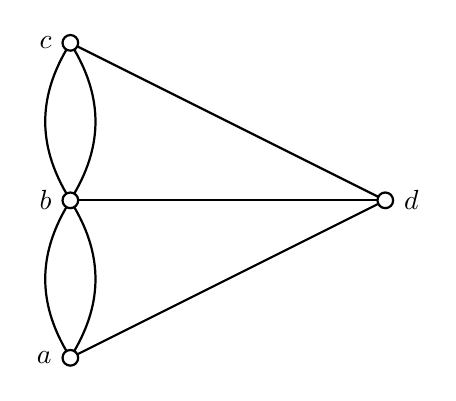
\begin{tikzpicture}[thick, main/.style = {draw, circle}]
        \node[main,scale=0.6, label=left:$a$] (a) at (0,0) {};
        \node[main,scale=0.6, label=left:$b$] (b) at (0,2) {};
        \node[main,scale=0.6, label=left:$c$] (c) at (0,4) {};
        \node[main,scale=0.6, label=right:$d$] (d) at (4,2) {};

        \draw (a) -- (d);
        \draw (b) -- (d);
        \draw (c) -- (d);
        \draw (a) to [out=120,in=240,looseness=1] (b);
        \draw (a) to [out=60,in=300,looseness=1] (b);

        \draw (b) to [out=120,in=240,looseness=1] (c);
        \draw (b) to [out=60,in=300,looseness=1] (c);

    \end{tikzpicture}
    \caption{The Seven Bridges of Königsberg}
\end{figure}

It was asked whether anyone could arrange a route in
such a way that he could cross each bridge once and
only once. Euler modelled the island and banks as
\emph{nodes}. Formally, this question asks if there is a cyclic
path that uses each edge once and only once. It turns out
there is provided the graph is connected and all nodes have
even degree.

Some terminology:

\begin{itemize}
    \item \textbf{Node}: Also known as points or vertices. Fundemental
          building block of a graph.
    \item \textbf{Edge}: Connects two nodes, or a node to itself.
    \item \textbf{Walk}: A sequence of vertices and edges, where the edges connect the adjacent vertices in the sequence.
    \item \textbf{Tour}: A walk with no repeated edges.
    \item \textbf{Path}: A walk with no repeated vertices. A \emph{simple} path has no repeated nodes.
    \item \textbf{Adjacent}: Said of two nodes connected by an undirected edge,
          or of the node to which a directed edges enters and the node of the edge's origin.
    \item \textbf{Degree}: Number of edges going out from a node. In a directed graph,
          there are both in and out degrees.
          \marginnote{Edges that go out from and enter the same node add two degrees to that node.}
    \item \textbf{Cycle}: A path from a node to itself. If there is a cycle in a
          graph, it is a cyclic graph. Else it is acyclic.
    \item \textbf{Connected}: An undirected graph is connected if every node can be reached
          from every other node. For a directed graph, the same property is called strongly connected.
\end{itemize}

Some notation: an undirected graph $G(V,E)$ consists of a set of nodes $V$
and edges $E$. Perhaps $V = {A, B, C}$ and $E = {(A,B), (A,A), (A, C)}$.
A directed graph $G<V, E>$ might have the same vertices, but edges
$E = {<A,B>, <A,A>, <A, C>}$ indicating that one may only travel from $A$
to other nodes.

There are two kinds of graph, \emph{directed} and \emph{undirected}.
In an undirected graph like the one shown previously, an edge can
go both ways. In a directed graph one can travel only one way along an
edge, represented by an arrow like in figure \ref{fig:directedgraph}

\begin{figure}
    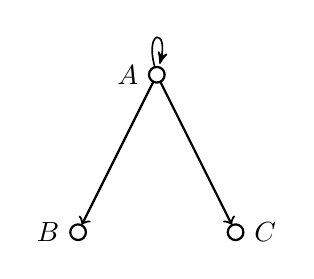
\begin{tikzpicture}[thick, main/.style = {draw, circle}]
        \node[main,scale=0.6, label=left:$A$] (a) at (0,2) {};
        \node[main,scale=0.6, label=left:$B$] (b) at (-1,0) {};
        \node[main,scale=0.6, label=right:$C$] (c) at (1,0) {};

        \draw[->] (a) -- (b);
        \path[->] (a) edge [loop above] ();
        \draw[->] (a) -- (c);

    \end{tikzpicture}
    \caption{Example of a Directed Graph}
    \label{fig:directedgraph}
\end{figure}

A \emph{weighted} graph has weights assocted with each directed edge. The weight
could represent probability of moving from one node to another, travel times, distances,
etc.

\subsection{Adjacency Matrix}

An \emph{adjacency matrix} is a way to represent a graph using a
2D array. For a graph with $n$ nodes, the adjacency matrix is an
$n \times n$ matrix where:

\begin{itemize}
    \item Each row and column corresponds to a node.
    \item The value at position $(i, j)$ is:
          \begin{itemize}
              \item $1$ (or the weight of the edge) if there
                    is an edge from node $i$ to node $j$.
              \item $0$ if there is no edge between node $i$ and node $j$.
          \end{itemize}
\end{itemize}

For an undirected graph, the adjacency matrix is symmetric,
meaning $A[i][j] = A[j][i]$. For a directed graph, the matrix
is not necessarily symmetric.

\textbf{Example:} Consider the directed graph in Figure
\ref{fig:directedgraph}. Its adjacency matrix is:

\[
    \begin{bmatrix}
        1 & 1 & 1 \\
        0 & 0 & 0 \\
        0 & 0 & 0
    \end{bmatrix}
\]

Here:
\begin{itemize}
    \item The value $1$ at $(1,1)$ represents the self-loop on $A$.
    \item The value $1$ at $(1,2)$ and $(1,3)$ represents edges from $A$ to $B$ and $A$ to $C$.
    \item All other entries are $0$ because there are no other edges.
\end{itemize}

\subsection{Linked List}

A \emph{linked list} representation of a graph uses an array of linked lists. Each node in the array represents a vertex, and the linked list at each index contains the neighbors of that vertex.

\textbf{Example:} Consider the directed graph in Figure \ref{fig:directedgraph}. Its linked list representation is:

\begin{itemize}
    \item $A \to A \to B \to C$
    \item $B \to \emptyset$
    \item $C \to \emptyset$
\end{itemize}

Here:
\begin{itemize}
    \item The first list represents the neighbors of $A$:
          a self-loop to $A$, and edges to $B$ and $C$.
    \item The second and third lists are empty because $B$ and
          $C$ have no outgoing edges.
\end{itemize}

The original nodes $A$, $B$, and $C$ can be stored in another
linked list, array, or whatever data structure is convenient.

\subsection{Graph Searching}

There are tow methods to traverse a graph.

\begin{itemize}
    \item Breadth First Search:
          A \emph{breadth first search} (BFS) visits all edges of distance $k$ from
          the source before visiting edges of distance $k+1$ from the source.
          Think of the waves rippling from a pebble thrown into a pond.
    \item Depth First Search:
          A \emph{depth first search} (DFS) visits one edge to the next node, then one edge from
          that node to the next. It goes downa  given path as far as possible
          before returning.
\end{itemize}

Breadth first lends itself to iteration, while depth first lends itself
to recursion.

\subsection{Shortest Path Algorithms}

There is a class of algorithms dedicated to finding the shortest 
path between two nodes, which broadly fall into two categories:
\begin{itemize}
    \item \emph{Greedy} algorithms
    \item \emph{Dynamic} algorithms
\end{itemize}
Greedy algorithms take the locally optimal choice at each step until they get to the 
node they're trying to reach, i.e. taking the shortest of two choices to get somewhere 
at each step. Dijkstra's algorithm is one such example of a greedy algorithm.
\begin{lstlisting}[caption={Dijkstra's algorithm}]
    Dijkstra(G, w, s) // s: starting node
        PQ <- V[G]
        for each node u in PQ
            d[u] <- infty; pred[u] <- NULL
        d[s] <- 0
        while PQ not empty
            u <- Extract-Min(PQ);
            for each node v in adj[u]
                if (v in PQ and d[v] > d[u] + w<u,v>)
                    d[v] <- d[u] + w<u,v>;
                    pred[v] <- u
\end{lstlisting}
Dijkstra's algorithm has a time complexity of $(V + E)\log(V)$. 

Dynamic algorithms create a decision tree and take the optimal path after exhaustively 
searching all possible paths. The Bellman-Ford algorithm is an example of a dynamic 
algorithm, and must be used to find the shortest path when negative edges are present.
\begin{lstlisting}[caption={Bellman-Ford algorithm}]
    Bellman-Ford(G, w, s) // s: source
        for each node u in V[G]
            d(0)[u] <- infty; pred(0)[u] <- NULL
        d(0)[s] <- 0
        for i <- 1 to |V[G]| - 1
            for each node u in V[G]
                d(i)[u] <- d(i-1)[u]
                pred(i)[u] <- pred(i-1)[u]
            for each edge <u,v> in E[G]
                if (d(i)[v] > d(i-1)[u] + w<u,v>)
                    d(i)[v] <- d(i-1)[u] + w<u,v>
                    pred(i)[v] <- u
        for each edge <u,v> in E[G]
            if (d(i)[v] > d(i)[u] + w<u,v>)
            return FALSE
        return TRUE
\end{lstlisting}

\section{Reference}
\begin{itemize}
    \item $E = mc^2$
\end{itemize}

\end{document}